%% This is an example first chapter.  You should put chapter/appendix that you
%% write into a separate file, and add a line \include{yourfilename} to
%% main.tex, where `yourfilename.tex' is the name of the chapter/appendix file.
%% You can process specific files by typing their names in at the 
%% \files=
%% prompt when you run the file main.tex through LaTeX.
\newcommand\mystrut{\rule[-0.9cm]{0pt}{2cm}}


\chapter{Enrichment and Homogenization Improvements}
The Results section showed that, for the problems run, the implementation of the hybrid method seems adequate to capture bulk behavior, like the end shape of a pile of collapsed grains. This however is interesting, as the previously described scheme includes a somewhat straightforward solution to ill-posed problems. The most ill-posed portion of the hybrid technique is the enrichment step, as a given continuum state can be represented by an infinite set of discrete element grain arrangements.

The solution applied to the enrichment problem, Avoid a Void, simply adds grains to all hybrid elements. There is no other information used to inform where Avoid a Void should place grains (as the Poisson Disk Sampling is random by nature), how many grains to add, or what kind of connectivity with other grains should be had. In the examples shown in the Results section, this is seemingly enough, as there are actually a relatively low number of conversions from discrete to continuum and continuum to discrete representations. For example, in the column collapse case, the core of the columns remain relatively steady, and conversion only happen around the exterior of the columns. Once the pile has collapsed, the pile remains steady and no other conversions occur. In the wheels driving over gravel example, there are also a lack of many conversions, as those conversions only occur for the elements directly under the wheel; once the wheel has driven past a set of elements, the granular bulk remains steady and the representations of the grains do not change.

The funnel flow example however indicates where the simple uninformed Avoid a Void scheme for enrichment can begin to break down. As can be seen in Figure \textcolor{red}{FINREFERENCE}, the top half of the funnel starts with both the pure discrete and hybrid funnels at the same volume. However after all of grains have flowed from the top half of the funnel to the bottom half, it can be clearly seen that the hybrid pile has lost volume compared to the pure discrete pile. The transient behavior is also different, with the hybrid scheme flowing at a different rate than the discrete grains. A key difference between the funnel flow geometry and the other previously discussed examples is that in the funnel flow, there is a continuous change from continuum to discrete grains at the top, and discrete to continuum grains at the bottom. The result is that the deficiencies of the enrichment and homogenization schemes are exposed. 

\section{Volume Change and Mass Conservation}

\begin{figure}[htp] 
    \centering
    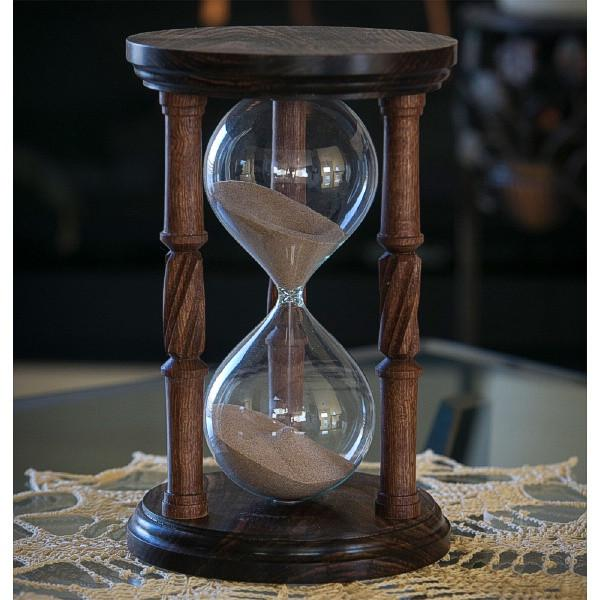
\includegraphics[width=0.4\textwidth]{figs/hourglass_whole.jpg}
    \caption{Mechanisms of deviations away from exact mass conservation.}
    \label{mass_change_mechanism}
\end{figure}

Every hybrid update step, the Avoid a Void scheme attempts to pack in grains in the hybrid elements. Because it does so in an uninformed matter however, this can lead to mass and volume loss or gain. For example, If the discrete grains in a hybrid cell have a large enough packing fraction $\Phi$ where the element remains hybrid, but below random close packing $\Phi_{RCP}$, the previously described enrichment scheme has a chance to pack in additional points. If that relatively low packing fraction is an accurate representation of the granular system at that element, then there may be mass introduced. If that hybrid element then is converted into a pure discrete element, permanent volume gain is then introduced into the system. 

On the other hand, mass can also be permanently lost in the system. If for a given hybrid element, the discrete grains have a packing fraction $\Phi < \Phi_{actual}$ based off of mass and volume that needs to be converted from a continuum representation, then the idea is that the Avoid a Void algorithm will eventually fill that missing space. However, Poisson Disk Sampling (PDS) has a limit and will not be able to reach $\Phi_{RCP}$. If $\Phi_{actual} \approx \Phi_{RCP}$ or worse, if $\Phi_{actual} \geq \Phi_{RCP}$ because the underlying discrete structure is crystalline, PDS will not be able to pack that space to the desired $\Phi$. In some geometries and flows, this may not be a problem, as, if the conversions happen at a slow rate compared to the hybrid update frequency, then the grains in an underpacked hybrid cell may rearrange to allow for PDK to pack in the enough grains. The column collapse and wheel examples for example, fall under this category. The funnel flow however has a continual flux of continuum into the hybrid zone which must be enriched. Mass loss occurs because the continuum to enrichment mass flux is larger than the source of discrete hybrid mass that the enrichment scheme can provide. The resulting lack of discrete particles then leads to volume loss.

\begin{figure}[htp] 
    \centering
    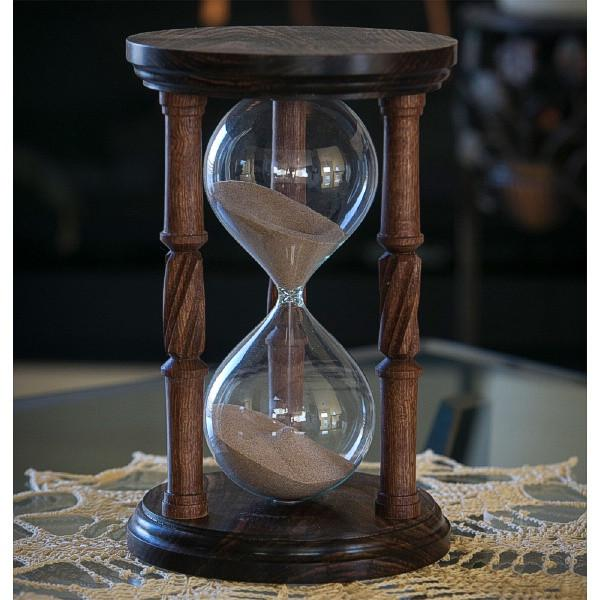
\includegraphics[width=0.4\textwidth]{figs/hourglass_whole.jpg}
    \caption{Evolution of a hybrid flow down a chute showing mass loss.}
    \label{chute_flow_old}
\end{figure}

As an extreme example, take the example of a flow down a chute with periodic boundary conditions. In this system, gravity is angled relative to the bottom boundary, driving continuous flow through the system. On the left side. discrete grains continuously enter a hybrid zone, where continuum points are in turn generated. As they move from left to right through the system, the discrete points are deleted as they enter the pure continuum zone and continuum points gain full weightage. The points then enter the hybrid zone on the right, where discrete grains are generated. Finally the continuum points exit into the discrete zone where they are deleted, and the discrete grains gain full weightage. With the current scheme, mass and volume are continuously lost. Eventually the pile of flowing grains reduces to a point where there is insufficient height to support a continuum or hybrid scheme according to the oracle, resulting in a pure discrete system.

There are thus two main problems that must be addressed: mass conservation and volume change tracking. These two problems however must be resolved in the discrete representation and continuum representation in different ways. Mass conservation for the continuum representation (converting mass from discrete grains to continuum) is fairly simple, as the continuum nature allows for mass addition or subtraction in whatever increments desired. Mass in the continuum can thus be tracked exactly over time. Volume change though must be conducted in a manner consistent with that mass change, and this must be addressed. 

For the discrete representation, mass conservation and volume change are completely coupled, as the density of the particles remains constant throughout the simulation. Mass conservation is more difficult to achieve in the discrete case, as mass conservation becomes a packing problem as previously described. Mass and volume in the discrete case also come in discrete units of a single grain at a time. This means that mass conservation cannot be exactly achieved in the discrete representation. The homogenization of a grain of radius $r_a$ can be offset by the enrichment of a grain of radius $r_b$, but mass will only be exactly conserved if $r_a = r_b$. For a monodisperse system this will of course always be true, but all the simulations run in this study have some polydispersity, making that condition almost never true. Thus mass conservation can only be achieved in a time-averaged sense for the discrete particle representation.

\subsection{Mass Ledger}

\begin{figure}[htp] 
    \centering
    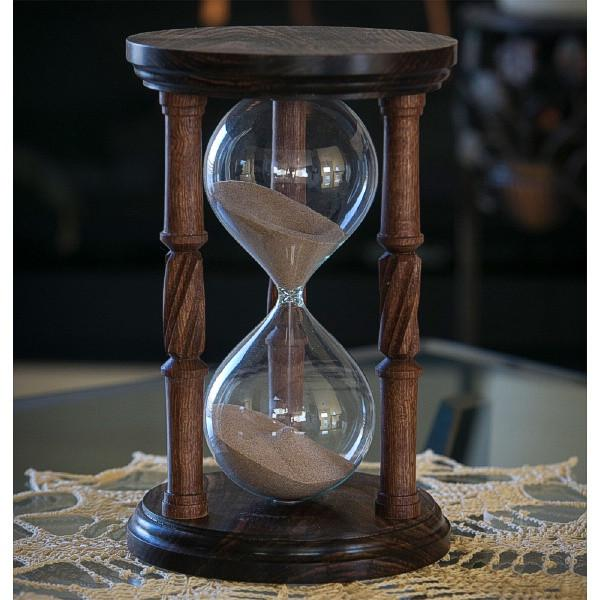
\includegraphics[width=0.4\textwidth]{figs/hourglass_whole.jpg}
    \caption{Mass fluxes in a hybrid system and the construction of a ledger.}
    \label{mass_ledger_schematic}
\end{figure}

In order to conserve mass and inform the enrichment scheme on how much mass must be converted from one representation to another, all of the relevant mass fluxes must be kept track of. Take as an example the simple hybrid system shown in Figure \ref{mass_ledger_schematic}. Again, a simple 50/50 weight split in the hybrid system is shown both for simplicity and to reflect the weight function used in the current study. At the $n^th$ timestep hybrid update, the marked DEM grain has radius $r_d$, density $\rho_d$, and weight $w^n_d=1$, resulting in a mass $m^n_d=m_d=w^n_d\rho_d\pi r^2_d$. At the $n^{n+1}$ hybrid update, the discrete grain $d$ has moved into the neighboring hybrid element (Element 1). Now, $w^{n+1}_d=0.5$, resulting in a mass $m^{n+1}_d=1/2m^{n}_d$. The mass difference $\Delta m_d=1/2m^d$ is mass that must be represented by continuum in order to maintain a partition of unity for the total mass that entered, $m_d$. There is thus a \textit{deficit} of continuum mass in Element 1 that must be added, through addition of mass to the currently existing MPM points, addition of a new MPM point with that deficit, or some combination of both.

Moving attention to the marked MPM point, the MPM point $p$ at the $n^th$ hybrid update is in the hybrid zone and has weight $w^n_p=0.5$ and mass $m^n_p=w^n_p m^p=0.5m^p$. At the next hybrid update its weight changes to 1, resulting in a mass of $m^{n+1}_p=m^p$ and a resulting continuum mass \textit{excess} in Element 2 of $0.5m^p$. 

From these cases it can be seen there are multiple ways that discrete and continuum mass can accrue deficits or excesses depending on weight changes as they move between different zone types. These excesses or deficits are logged in a mass \textit{ledger}, which informs the enrichment and homogenization schemes on how much mass of which type of representation is required. It should be noted that while there must always be at least one hybrid zone between a pure discrete and pure continuum zone, a grain in a pure discrete zone at hybrid update step $n$, it is still possible for it to advect to a pure continuum step $n$ due to geometry and hybrid update frequency. This can be seen in Figure \ref{pure_dem_to_continuum}.

\begin{figure}[htp] 
    \centering
    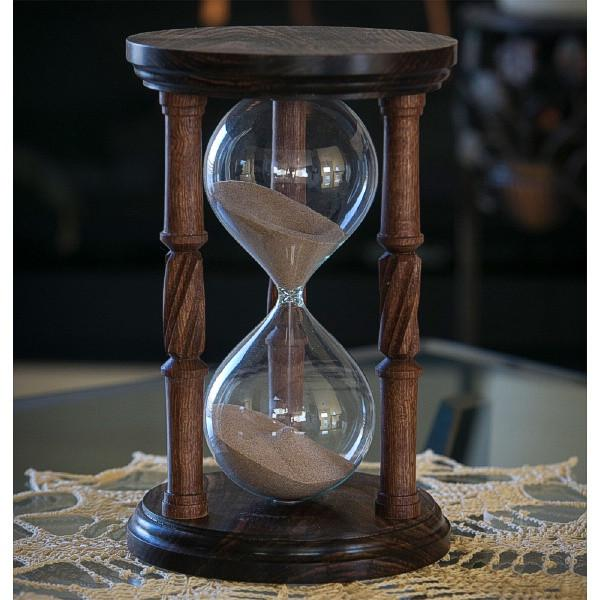
\includegraphics[width=0.4\textwidth]{figs/hourglass_whole.jpg}
    \caption{Discrete particle entering a pure continuum regime.}
    \label{pure_dem_to_continuum}
\end{figure}

This case is not treated any differently to the previously described cases. While the discrete point is deleted from the system for being in a pure continuum zone, this can be interpreted as simply a weight change from $w_d=1$ to $w_d=0$. This results in a continuum mass deficit of $m_d$ in the element that the grain was deleted from. The same could of course occur for an MPM point entering a pure discrete region, resulting in a discrete mass deficit.

This analysis so far has assumed a fixed domain decomposition, where all element types remain fixed over time. This however does not need to be the case, as the framework of mass deficits or excesses as a result of weight changes can generalize to a system where DEM grains and MPM points advect through elements with different representations, as well as the representations themselves changing from timestep to timestep. For the mass ledger, all that needs to be known is the type of zone that the grain or point was in at the previous hybrid update, and what type of zone it is currently in. If the zone type was the same for the starting element at the previous update as the current element at the current update, then no change to the ledger needs to be made. If the zone types are different, then the mass difference due to the weight change is then marked in the ledger.

\subsection{Mass Ledger Implementation}
In order to keep track of mass deficits or excesses, two ledgers are introduced, which, in implementation, are simple vectors: the \textbf{dem\_deficit} and \textbf{continuum\_deficit}. Each vector stores the eponymous mass deficit on each element in the simulation. To establish convention, mass deficits are positive and excesses are negative. Assuming an MPM point starting with a mass $m_p$ and a DEM grain with mass $m_d$, the ledger changes can be summarized as:

\def\Zones{\makecell[tl]{Discrete\\ Continuum\\ Hybrid\\ \\ Discrete\\ Continuum\\ Hybrid}}
\def\demdeficit{\textbf{dem\_deficit}}
\def\mpmdeficit{\textbf{mpm\_deficit}}

\begin{table}
  \centering
  \footnotesize
  \renewcommand{\cellalign}{lc}
  \begin{tabular}{lllll}
    \toprule
    Representation & Start Zone & End Zone & Ledger & Deficit  \\
    \midrule
    DEM Grain & \makecell[tl]{Discrete\\ \\ \\ \\Hybrid} & \Zones & \makecell[tl]{N/A\\ \mpmdeficit\\ \mpmdeficit\\ \\ \mpmdeficit\\ \mpmdeficit\\ N/A} & \makecell[tl]{N/A\\ $+m_d$\\ $+0.5m_d$\\ \\ $-0.5m_d$\\ $+0.5m_d$\\ N/A} \\
    \midrule
    MPM Point & \makecell[tl]{Continuum\\ \\ \\ \\Hybrid} & \Zones & \makecell[tl]{\demdeficit\\ N/A\\ \demdeficit\\ \\ \demdeficit\\ \demdeficit\\ N/A} & \makecell[tl]{$+m_p$\\ N/A\\ $+0.5m_p$\\ \\ $+0.5m_p$\\ $-0.5m_p$\\ N/A} \\
    \bottomrule
  \end{tabular}
  \caption{Mass ledger contributions.}
  \label{mass_ledger_table}
\end{table}

The mass ledgers for a hybrid update are calculated near the beginning of the hybrid update: it is done after the level set calculation and after the oracle has determined the zone types based on those calculations, but before the enrichment and homogenization steps. The ledgers are updated every hybrid update, so that there is a running list of mass deficits. This thus enables a way to prevent mass gain and tackle mass loss. If an element has a negative deficit due to, for example, introducing a grain with a slightly larger radius than was needed, then the ledger can inform the enrichment scheme to not introduce any more DEM grains in that cell. On the other hand, if there is a positive deficit, then if at a given hybrid update the packing scheme is unable to introduce enough grains, then there is a chance in future updates that the grains have reached a configuration to allow for further grain introduction. Implementation wise, only elements that have a positive deficit are marked for enrichment.

\section{Packing Schemes}
Practically speaking, the mass ledger mostly addresses mass gain problems, as it stops enrichment in those elements. In elements that have a deficit, the enrichment scheme will continuously try to input grains and points, but this is not any different than the previously used scheme which tried to pack grains for all hybrid elements at every hybrid update. The problem remains that for certain geometries and flow profiles, the Avoid a Void's PDS scheme, which is random in nature, was unable to introduce DEM grains at a high enough packing fraction at a rate equal to or greater than the continuum mass flux into a hybrid cell. A new packing scheme is needed. The following section summarizes the different packing strategies that were attempted and discusses their characteristics.

In order to evaluate the effectiveness of new packing schemes, the inclined plane geometry shown in Figure \ref{chute_flow_old} is used as a case study. The hyperelastic model was used to obtain the result shown in Figure \ref{chute_flow_old} for demonstration purposes; a switch is now made to the hypoelastic model, as it includes the $\mu(I)$ relation that captures the correct velocity profile in an inclined chute flow, minimizing the role of the constitutive law in the mass loss issue.

\subsection{Random Packing}
Before any new packing methodologies are introduced however, it should be noted that the random scheme has a parameter \textit{numTrials} which controls the number of attempts the code makes to introduce a new point. For all of the simulations shown in the Results section, this was set to 20, mostly as a compromise between speed and accuracy for the geometries that we. The first logical attempt at a solution to the packing problem is then to simply increase the number of attempts, trading the time lost in increasing the number of attempts for better packing. 

\begin{figure}[htp] 
    \centering
    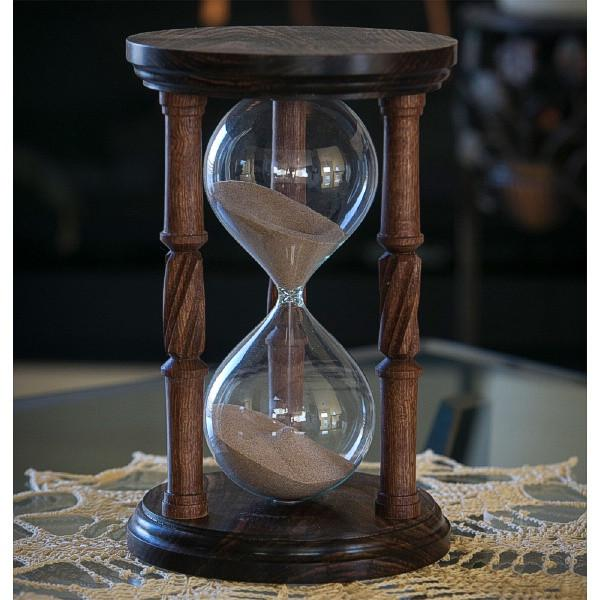
\includegraphics[width=0.4\textwidth]{figs/hourglass_whole.jpg}
    \caption{Mass over time for random packing.}
    \label{mass_time_random}
\end{figure}

As Figure \ref{mass_time_random} shows, this is not enough. While increasing \textit{numTrials} does help slow down the mass loss rate, the mass loss rate does reach a limit as a function of \textit{numTrials}. At first pass this may seem counterintuitive, as in the limit of infinite trials a dense configuration should be sampled. However, this is not true do the fact that the random packing scheme is a greedy scheme. If the random scheme picks a point center with a random radius that has no collisions with any other point in the enriched element, then that point will be considered valid and added to the existing points. This limits the possible areas that new grains can now enter, as can be seen in Figure \ref{greedy_dem}. 

\begin{figure}[htp] 
    \centering
    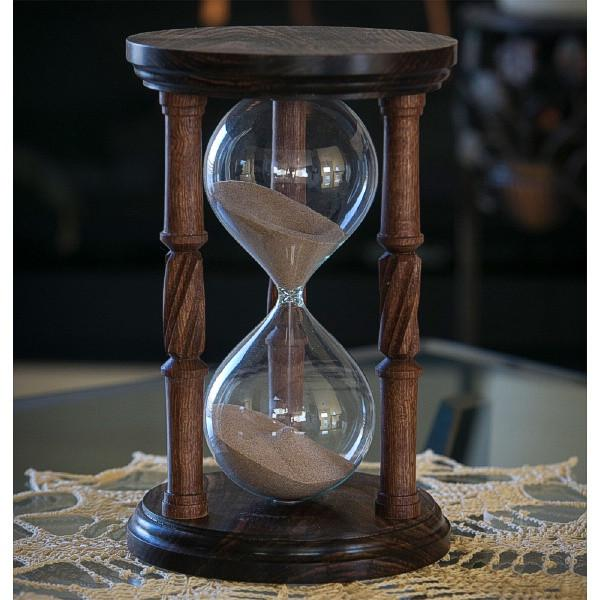
\includegraphics[width=0.4\textwidth]{figs/hourglass_whole.jpg}
    \caption{Non-optimal grain placement leading to inability to reach target packing fraction.}
    \label{greedy_dem}
\end{figure}

\subsection{Grid Packing}
Enrichment can occur often, depending on the geometry of the problem. Because of this, speed is still a requirement of any practical packing scheme. Thus, while less informed greedy schemes may not provide adequete packing, they do potentially show a much larger speed advantage over other schemes. Packing in general is a problem that shows up in many contexts, and solutions do exist that show the ability to attain very high packing fractions that still avoid crystalline packings \textcolor{red}{FINDREFERENCE}. However these solutions are currently avoided, due to their computational expense. For example, some class of solutions solve a constrained minimization problem, maximizing packing fraction while constrained to limited or no overlaps. Introducing an optimization solve is potentially too slow for the current application. On the other hand there are a class of solutions that essentially inject grains at random in a system and substep a discrete element method to attain a viable configuration. Again, solving a sub discrete element problem with multiple timesteps needed to achieve an equilibrium state is too expensive.

\begin{figure}[htp] 
    \centering
    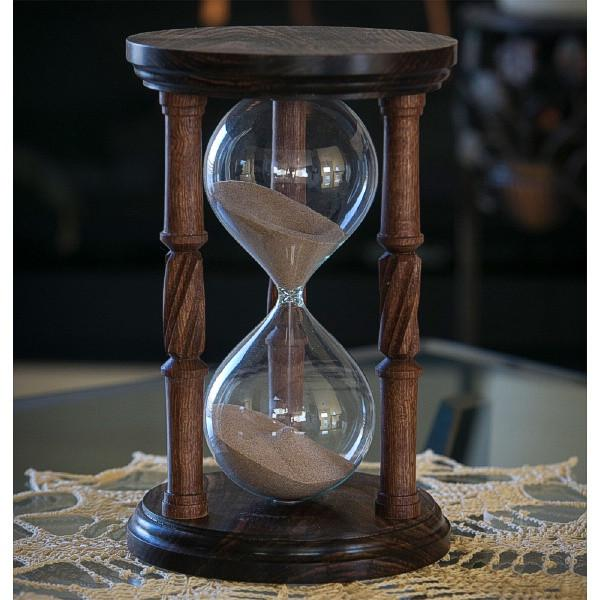
\includegraphics[width=0.4\textwidth]{figs/hourglass_whole.jpg}
    \caption{Chute flow example zoomed into hybrid zone.}
    \label{chute_flow_old_closeup}
\end{figure}

Therefore, a more guided greedy method is desired. From Figure \ref{chute_flow_old} it can be seen that as the grains flow from left to right, space intuitively opens up upstream of the hybrid elements. The next solution attempted utilized this fact, prioritizing grain injection attempts to the downstream-most available spaces in the element, to promote closer packing to the currently existing grains. To do this, the area of an enriched hybrid element was discretized into a grid. The nodes of the grid represent possible injection points. As a note, this presents a parameter that must be tuned: the discretization distance between nodes. Smaller discretizations can lead to less space between injected points, but also increases the number of attempts that must be made. 

\begin{figure}[htp] 
    \centering
    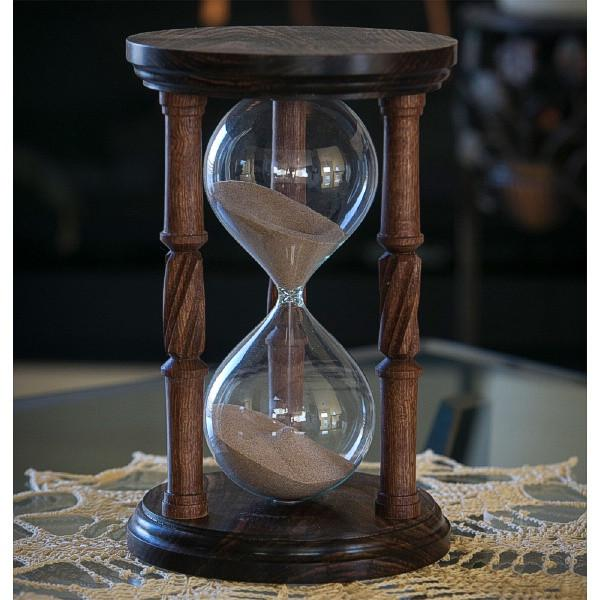
\includegraphics[width=0.4\textwidth]{figs/hourglass_whole.jpg}
    \caption{Grid enrichment scheme.}
    \label{grid_enrichment}
\end{figure}

The scheme would then attempt to inject grains, starting from the downstream side. The downstream direction was determined by checking the surrounding elements of the element currently being enriched; if a continuum element neighbors the hybrid element, then the downstream element side is the side opposite of the shared element side. If a discrete element is adjacent to the enriched element, then that face is taken as the downstream side. If only hybrid elements surround the current element, then a direction is picked at random. 

\subsection{Circle Sweep}
\def\seed{\textbf{seed\_queue}}
While the grid scheme was an improvement over the initial random packing, it proved to still be unable to provide a discrete mass source that offset the continuum mass flux into a hybrid cell. The goal of the scheme was to increase the chances of introducing points closer to the existing points; this was achieved, but not to the desired level. To address this deficiency, the next scheme, deemed here the "circle sweep" scheme, strictly forced at least one point of tangency for any injected grain to the other grains in the cell.

\begin{figure}[htp] 
    \centering
    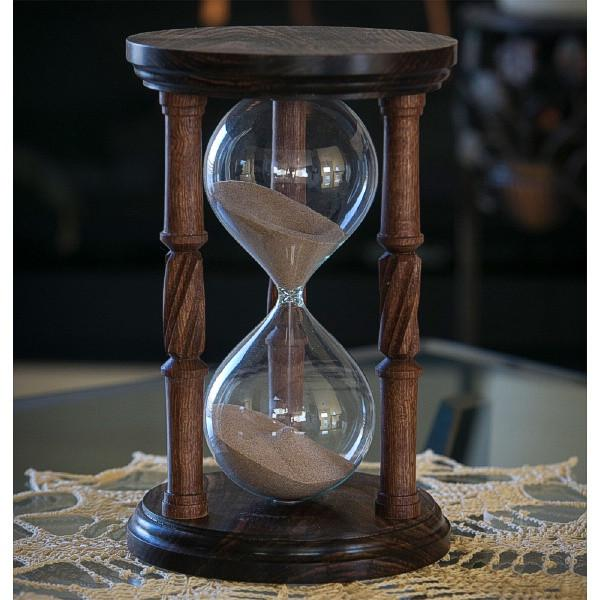
\includegraphics[width=0.4\textwidth]{figs/hourglass_whole.jpg}
    \caption{Circle sweep scheme.}
    \label{circle_sweep_enrichment}
\end{figure}

In order to discuss the scheme, take as an example a pure continuum element that at the current hybrid update is now a hybrid cell, and must be enriched. To initialize the scheme, a grain is injected at a random location within the element and is given an index number $i$ of 1. This index number is added to a queue of indices called the \seed. The angular space \textcolor{red}{FINDTERM} of 2$\pi$ around this grain is then discretized into $n$ angular divisions. Grains injections are then attempted at all of these angular divisions at a distance equal to the sum of the radius of the seed grain $r_i$ and the new grain $r_{new}$, assuring that any new grain has at least one point of tangency to other grains in the element. A new valid grain is given an index number of 1 plus the index number of the grain at the rear of the queue, which itself is then enqueued. Once injection attempts have been made at all of the possible angles around the seed grain, the index of the seed grain is dequeued. The next grain in the \seed then becomes the seed grain, and the process is continued. The scheme then stops once the queue is empty.

In hybrid elements with DEM grains already present, the circle sweep algorithm begins by enqueueing all of those grains in the \seed, instead of injecting a grain at random to initialize the queue. The algorithm then continues as stated, working through the \seed. Again, this scheme introduces a tunable parameter $n$, which controls the number of injection attempts made around every seed grain.

\subsection{Two Point Tangent}
The circle sweep scheme represents an improvement over the grid scheme, but again, for the chute flow geometry was not enough to offset the continual continuum mass flux into the hybrid elements. The final scheme attempted, called the "two-point-tangent" (TPT) scheme, as its name suggests, enforces two points of tangency for any new injected points. 

In order to initialize the TPT scheme for a newly enriched element, a grain is injected at random and added to the same \seed data structure as the circle sweep scheme. The angular region around the grain is again discretized and grain injections are attempted at these angles. The divergence point between TPT and the circle sweep scheme occurs when a valid grain is found and added to the \seed. Instead of continuing injection attempts at the other remaining possible angles, the scheme stops, and uses these two grains as the starting point of the scheme. With these two tangent grains of radius $r_a$ and $r_b$, a new grain with radius $r_c$ can be injected that is tangent to both of the first two. Given the center points of the grains $a$ and $b$ and their radii, and the radius of the new grain $r_c$, an analytical formula can be derived for the two possible center points of the new grain $c$ that maintains tangency with $a$ and $b$. Injection attempts are then made at these two locations, and any valid attempts are added to the simulation and to the \seed.


\subsection{Packing Scheme Results}


\section{Hypoelastic Pressure Update}

